\documentclass[12pt]{beamer}
\title{Cultura política y Apoyo a la Democracia en Chile}
\subtitle{Un análisis desde las juventudes en 2021}
\author{Ignacio Tapia Fuentes}
\institute{Profesor guía: Rodrigo Medel Sierralta \and
Profesora informante: Federica Sánchez Staniak \and
Ayudante de cátedra: Camila Rodríguez Peña}
\date{\today}

\begin{document}
\begin{frame}
\titlepage
\begin{figure}
\centering
\includegraphics[height=1.5cm]{images/logo.png}
\end{figure}
\end{frame}

\begin{frame}
\frametitle{Tabla de contenidos}
\tableofcontents
\end{frame}

\begin{frame}
\frametitle{1. Presentación}
\begin{itemize}
\item ¿Qué anima esta investigación?
\item ¿Por qué estudiar la cultura política y el apoyo a la democracia en las juventudes?
\end{itemize}
\end{frame}

\begin{frame}
\frametitle{Problematización}
\begin{itemize}
\item El estilo tecnocrático de la política chilena post transición
\item La crisis de representatividad de los partidos políticos
\item La democracia incompleta
\item El desencuentro entre la política institucional y la ciudadanía en su conjunto y los efectos de esta situación en los efectos de los jóvenes hacia la democracia
\end{itemize}
\end{frame}

\begin{frame}
\frametitle{3. Pregunta de investigación}
\begin{itemize}
\item ¿Cómo se caracterizan los indicadores de cultura política y apoyo a la democracia en las juventudes chilenas durante 2021?
\end{itemize}
\end{frame}

\begin{frame}
\frametitle{Objetivos}
\begin{itemize}
\item  Objetivo general: Conocer la distribución de distintos indicadores de cultura política y su relación con el apoyo a la democracia.
\item Objetivos específicos:
\item Describir el estado actual de indicadores de cultura política asociados a conocimiento e interés en la política.
\item  Describir el estado actual de indicadores de cultura política asociados a confianza institucional.
\item Describir el estado actual de indicadores de cultura política asociados a percepciones hacia la democracia.
\end{itemize}
\end{frame}

\begin{frame}
\frametitle{Métodos}
\begin{itemize}
\item Datos utilizados
\item Unidad de observación
\item Técnicas de análisis a utilizar
\item Matriz de operacionalización
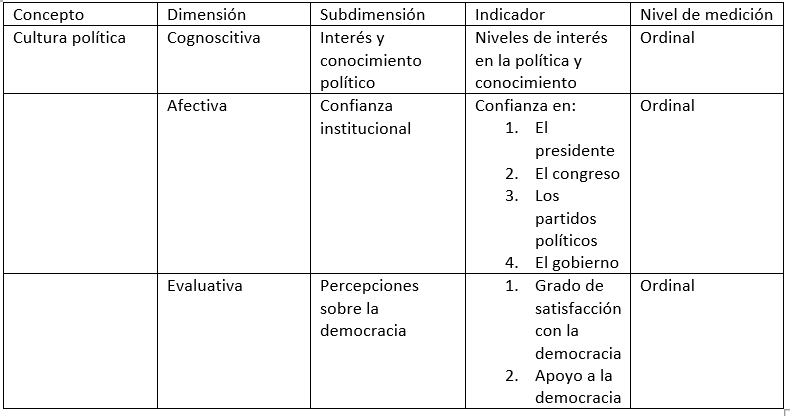
\includegraphics[height=5cm]{images/tabla.PNG}
\end{itemize}
\end{frame}

\begin{frame}
\frametitle{Hallazgos}
\begin{itemize}
\item Descriptivos de frecuencia para la dimensión "Percepciones hacia la democracia"
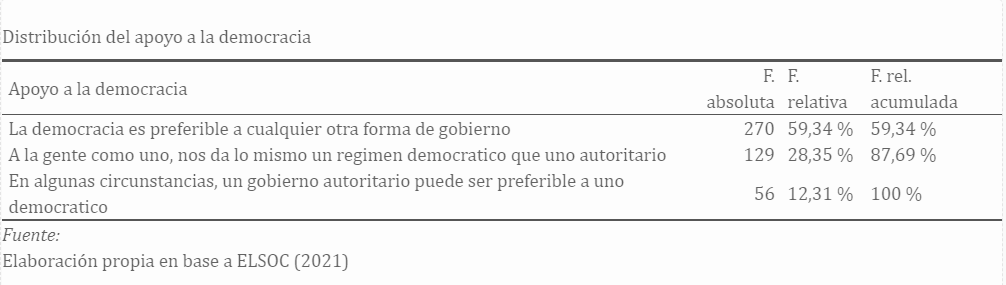
\includegraphics[height=3cm]{images/tabla frecuencia apoyo_dem.PNG}
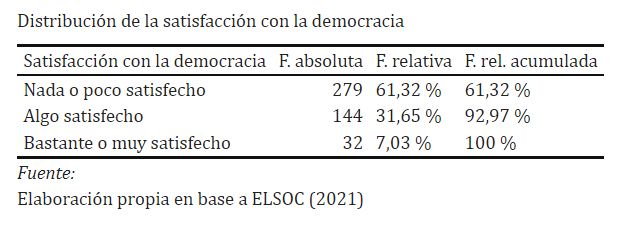
\includegraphics[height=3cm]{images/tabla frecuencia satis_dem.PNG}
\end{itemize}
\end{frame}

\begin{frame}
\frametitle{Hallazgos}
\begin{itemize}
\item Descriptivos de frecuencia para la dimensión de 
 "Interés político"
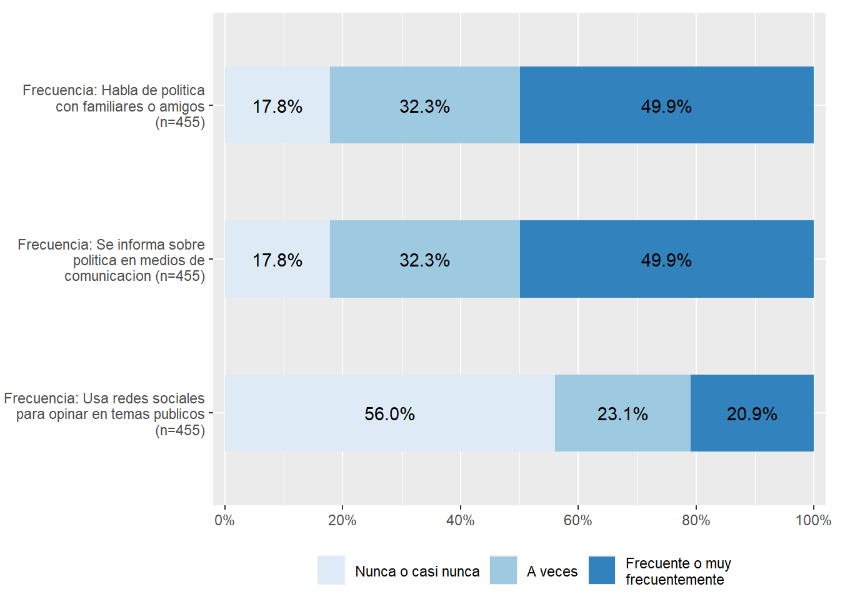
\includegraphics[height=6cm] {images/conocimiento_frq.PNG}
\end{itemize}
\end{frame}

\begin{frame}
\frametitle{Hallazgos}
\begin{itemize}
\item Descriptivos de frecuencia para la dimensión de "Confianza institucional"
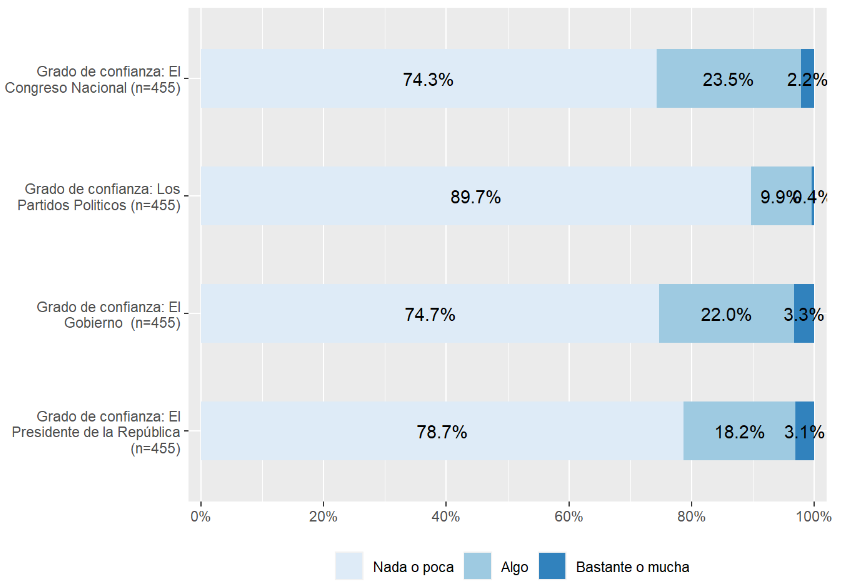
\includegraphics[height=6cm] {images/indicadores_confianza.PNG}
\end{itemize}
\end{frame}

\end{document}